\documentclass{article}

\usepackage[final]{neurips_2019}
\usepackage{amsmath}
\usepackage[utf8]{inputenc}
\usepackage[T1]{fontenc}
\usepackage{hyperref}
\usepackage{url}
\usepackage{booktabs}
\usepackage{amsfonts}
\usepackage{nicefrac}
\usepackage{microtype}
\usepackage{graphicx}
\usepackage{xcolor}
\usepackage{tabularx}
\usepackage{float}
\usepackage{pifont}
\usepackage[normalem]{ulem}
\usepackage{tikz}


\usepackage{enumitem}
\usetikzlibrary{shapes.geometric, arrows, positioning, fit, backgrounds}
\newcommand{\cmark}{\ding{51}}
\newcommand{\xmark}{\ding{55}}

\title{
  SLM-Math: Empowering Small Language Models for Mathematical Reasoning \\
  \vspace{1em}
  \small{\normalfont Columbia COMS4705 Final Project Report} \\
  \small{\normalfont \textbf{Keywords:} \textit{Small Language Models, Reinforcement Learning, Mathematical Reasoning, Multi-Agent Systems, Chain-of-Thought}}
}

\author{
  Roger Wang \\
  Department of Computer Science \\
  Columbia University \\
  \texttt{lw3240@columbia.edu} \\
  \And
  Jinzi Luo \\
  Department of Computer Science \\
  Columbia University \\
  \texttt{jl7199@columbia.edu} \\
  \And
  Yunchen Yuan \\
  Department of Computer Science \\
  Columbia University \\
  \texttt{yy3610@columbia.edu} \\
}

\raggedbottom

\renewcommand{\topfraction}{0.9}
\renewcommand{\bottomfraction}{0.9}
\renewcommand{\textfraction}{0.1}
\renewcommand{\floatpagefraction}{0.8}
\setcounter{topnumber}{3}
\setcounter{bottomnumber}{3}
\setcounter{totalnumber}{5}

\begin{document}

\maketitle

\begin{abstract}
We investigate enhancing a 1.5B-parameter model (Qwen2.5-Math-1.5B) for mathematical reasoning through: (1) chain-of-thought data generation via Grok-4.1-Fast and MiniMax-M2, (2) supervised fine-tuning (SFT) with full and LoRA configurations, (3) GRPO reinforcement learning, and (4) ten agentic workflow architectures. SFT LoRA achieves 80.0\% on GSM8K-test (+14.2 percentage points over 65.8\% base), GRPO reaches 82.4\% (+2.4 percentage points), and Solver--Verifier (SFT both) achieves 86.4\% (+20.6 percentage points). Cross-dataset transfer to MATH-500 shows consistent gains (67.2\% versus 53.2\% base). A key observation is that the model spontaneously generates Python code during reasoning but fails to mentally execute it correctly; our code-executing agents address this by extracting and running the model's own code, yielding substantial accuracy improvements. Our findings demonstrate complementary roles of training-time supervision, reinforcement learning, and inference-time verification for small language models.
\end{abstract}

\section{Key Information}
\textbf{Team:} Roger Wang (lw3240), Jinzi Luo (jl7199), Yunchen Yuan (yy3610). \textbf{TA mentor:} Melody Ma. \textbf{External collaborators:} None. \textbf{Project sharing:} COMS4705 only.

\section{Introduction}

Large language models achieve strong mathematical reasoning but are impractical for widespread deployment due to computational cost. We investigate enhancing Qwen2.5-Math-1.5B~\cite{yang2024qwen2}---a 1.5B-parameter math-specialized model---through supervised fine-tuning (SFT), GRPO reinforcement learning~\cite{shao2024deepseekmath}, and agentic workflows. We evaluate on GSM8K~\cite{cobbe2021training} (grade-school arithmetic) and MATH~\cite{hendrycks2021measuring} (competition-level problems).

\textbf{System Design.} Our pipeline (Figure~\ref{fig:pipeline}): Base model $\rightarrow$ SFT (LoRA~\cite{hu2021lora}/Full) $\rightarrow$ optional GRPO RL $\rightarrow$ agentic workflows. Agents can operate on \textit{any} checkpoint---we evaluate base, SFT, and RL models with various agent architectures to understand which combinations work best and why.

\begin{figure}[!htbp]
\centering
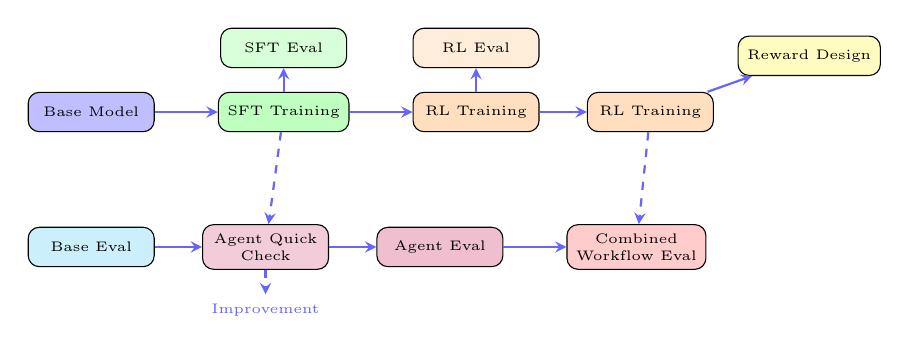
\begin{tikzpicture}[
  node distance=0.4cm and 0.6cm,
  box/.style={rectangle, draw, rounded corners, minimum width=1.6cm, minimum height=0.5cm, align=center, font=\tiny},
  arrow/.style={->, >=stealth, thick, blue!60}
]
% Training Pipeline (top row)
\node[box, fill=blue!25] (base) {Base Model};
\node[box, fill=green!25, right=0.8cm of base] (sft) {SFT Training};
\node[box, fill=green!15, above=0.3cm of sft] (sfteval) {SFT Eval};
\node[box, fill=orange!25, right=0.8cm of sft] (rl1) {RL Training};
\node[box, fill=orange!15, above=0.3cm of rl1] (rleval) {RL Eval};
\node[box, fill=orange!25, right=0.6cm of rl1] (rl2) {RL Training};
\node[box, fill=yellow!25, above right=0.2cm and 0.3cm of rl2, font=\tiny] (reward) {Reward Design};

% Evaluation Pipeline (bottom row)
\node[box, fill=cyan!20, below=1.2cm of base] (baseeval) {Base Eval};
\node[box, fill=purple!20, right=0.6cm of baseeval] (agentcheck) {Agent Quick\\Check};
\node[box, fill=purple!25, right=0.6cm of agentcheck] (agenteval) {Agent Eval};
\node[box, fill=red!20, right=0.8cm of agenteval] (combined) {Combined\\Workflow Eval};

% Arrows - Training
\draw[arrow] (base) -- (sft);
\draw[arrow] (sft) -- (sfteval);
\draw[arrow] (sft) -- (rl1);
\draw[arrow] (rl1) -- (rleval);
\draw[arrow] (rl1) -- (rl2);
\draw[arrow] (rl2) -- (reward);

% Arrows - Evaluation
\draw[arrow] (baseeval) -- (agentcheck);
\draw[arrow] (agentcheck) -- (agenteval);
\draw[arrow] (agenteval) -- (combined);

% Cross-pipeline arrows
\draw[arrow, dashed] (sft) -- (agentcheck);
\draw[arrow, dashed] (rl2) -- (combined);
\draw[arrow, dashed] (agentcheck) -- ++(0,-0.6) node[below, font=\tiny] {Improvement};

\end{tikzpicture}
\caption{System pipeline: Training flow (top) includes SFT and iterative RL with evaluation checkpoints. Evaluation flow (bottom) tests agents on different model checkpoints and combines workflows for final assessment.}
\label{fig:pipeline}
\end{figure}

\textbf{Contributions.} (1) A unified comparison of SFT, RL, and agentic workflows for small math-specialized models. (2) 14--21 percentage point accuracy gains through combined training and inference strategies. (3) Analysis of why some agents hurt small model performance. (4) Evidence that simple Solver--Verifier architectures outperform complex tool-based approaches for capacity-limited models.

\section{Related Work}

\textbf{Math-Specialized Models and SFT.} Domain-specific pretraining improves reasoning performance at small scales~\cite{yang2024qwen2,wang2023mathcoder}. Chain-of-thought prompting~\cite{wei2022chain} enables step-by-step reasoning transfer via teacher-student fine-tuning. We compare full SFT versus LoRA~\cite{hu2021lora} and demonstrate cross-dataset transfer.

\textbf{Reinforcement Learning for Reasoning.} GRPO~\cite{shao2024deepseekmath} optimizes correctness beyond imitation learning. Process supervision~\cite{lightman2023lets} rewards intermediate steps but requires extensive annotation. We apply GRPO with binary rewards, showing gains when combined with SFT initialization.

\textbf{Agentic Reasoning.} Solver--Checker architectures~\cite{wu2023mathchat}, self-consistency~\cite{wang2022selfconsistency}, and program-aided reasoning~\cite{gao2023pal} allow models to verify or refine reasoning. We design lightweight workflows for small models, finding simple verification outperforms complex pipelines.

\section{Approach}
\label{sec:approach}

\subsection{Baseline Model}
We selected Qwen2.5-Math-1.5B~\cite{yang2024qwen2} after experimenting with alternatives. General-purpose models (Qwen2.5-1.5B, Qwen2.5-0.6B) showed limited responsiveness to agentic workflows. Qwen2.5-Math-1.5B offered a middle ground: small enough to benefit from our methods, yet strong enough for multi-step reasoning.

\subsection{Data Pipeline}
We generate CoT data using a two-round cascade: Grok-4.1-Fast (primary, 3 attempts) followed by MiniMax-M2 (backup, 5 attempts for failed problems). Each attempt produces structured output: \texttt{<think>...</think>} reasoning ending in \(\boxed{\text{answer}}\). Only solutions matching ground truth are retained. From 19,473 training samples (7,473 GSM8K~\cite{cobbe2021training} + 12,000 MATH~\cite{hendrycks2021measuring}), we obtain 18,946 verified CoT samples (97.3\% success rate). Table~\ref{tab:data-stats} shows statistics.

\begin{table}[!htbp]
\centering
\caption{Generated chain-of-thought data statistics by source dataset.}
\label{tab:data-stats}
\small
\begin{tabular}{lccccc}
\toprule
\textbf{Dataset} & \textbf{Total Problems} & \textbf{Successful} & \textbf{Success Rate} & \textbf{Average Length} & \textbf{With Code} \\
\midrule
GSM8K & 7,473 & 7,298 & 97.7\% & 320 tokens & 45\% \\
MATH & 12,000 & 11,648 & 97.1\% & 480 tokens & 72\% \\
\bottomrule
\end{tabular}
\end{table}

\subsection{Supervised Fine-Tuning}
We train in two configurations: \textbf{Full SFT} (learning rate $5\times10^{-5}$, all parameters) and \textbf{LoRA}~\cite{hu2021lora} (rank 16, learning rate $1\times10^{-4}$, adapter weights only). Both use cosine scheduling, bfloat16, batch size 128, for 2 epochs. LoRA rank 16 was chosen via ablation: rank 8 underperformed by 2.1 percentage points; rank 32 provided no gain. Training demonstrates transfer from GSM8K to MATH-500.

\subsection{Reinforcement Learning with GRPO}

Reinforcement learning is a core component of our pipeline, applied after SFT to directly optimize for answer correctness. We use Group Relative Policy Optimization (GRPO)~\cite{shao2024deepseekmath}, which computes advantages by comparing responses within each batch rather than requiring a separate value network.

\textbf{Training Configuration.} We initialize from the SFT LoRA checkpoint and train with the following hyperparameters:
\begin{itemize}[nosep,leftmargin=*]
\item Learning rate: $5\times10^{-6}$ with cosine decay to $1\times10^{-7}$
\item Batch size: 16 prompts per step, $K=2$ responses per prompt (32 total generations)
\item Gradient accumulation: 4 steps (effective batch size 64)
\item KL coefficient: $\beta=0.05$
\item Training duration: 1 epoch on GSM8K (7,473 problems, approximately 470 optimization steps)
\item Optimizer: AdamW with weight decay 0.01
\end{itemize}

\textbf{Reward Function Design.} We use a structured reward function with three components:
\begin{enumerate}[nosep,leftmargin=*]
\item \textbf{Correctness reward} ($w_{\text{correct}}=1.0$): $+1.0$ for exact match with ground truth after normalization, $-1.0$ for mismatch.
\item \textbf{Format reward} ($w_{\text{format}}=0.1$): $+0.1$ for properly formatted \(\boxed{}\) answer, $-0.1$ for missing or malformed format.
\item \textbf{Parsing penalty} ($w_{\text{parse}}=0.5$): $-0.5$ for completely unparsable outputs (no extractable answer).
\end{enumerate}
The total reward is: $r = w_{\text{correct}} \cdot r_{\text{correct}} + w_{\text{format}} \cdot r_{\text{format}} + w_{\text{parse}} \cdot r_{\text{parse}}$. This formulation encourages both correct answers and proper formatting while penalizing outputs that cannot be evaluated.

\textbf{Answer Extraction and Normalization.} We extract answers from \(\boxed{}\) format using balanced brace matching, with fallback to ``Final Answer:'' or last numeric value. Normalization includes lowercase conversion, LaTeX command removal, comma/whitespace stripping, and fraction-to-decimal conversion.

\textbf{KL Regularization.} The loss function is $\mathcal{L}_{\text{GRPO}} = -\mathbb{E}[\hat{A}(x,y) \cdot \log \pi_{\theta}(y|x)] + \beta \,\mathrm{KL}(\pi_{\theta} \| \pi_{\text{ref}})$ where $\hat{A}(x,y)$ is the advantage computed relative to other responses in the batch. We found $\beta=0.05$ optimal: $\beta=0$ caused reward hacking; $\beta=0.1$ over-constrained updates.

\textbf{Training Dynamics and Results.} GRPO provides +2.4 percentage points over SFT (82.4\% versus 80.0\% on GSM8K). Training requires 4--6 hours on NVIDIA H20. Key observations: (1) RL gains require high-quality SFT initialization---applying GRPO to base model yields unstable training. (2) $K=2$ responses per prompt balances exploration with compute; $K=1$ provides insufficient variance, $K=4$ shows no proportional gains. (3) Most improvement occurs in the first 200 steps; later training provides diminishing returns.

\subsection{Agentic Workflows}

We implement training-free inference-time agents that can operate on \textit{any} model checkpoint (base, SFT, or RL). This flexibility allows us to study how training improvements interact with workflow designs. In our experiments, we evaluate each agent architecture on multiple checkpoints---Table~\ref{tab:main-results} specifies which checkpoint each configuration uses. Table~\ref{tab:agent-descriptions} describes each architecture; Figures~\ref{fig:solver-verifier} and~\ref{fig:code-feedback} illustrate the two most effective workflows.

\begin{table}[!htbp]
\centering
\caption{Agentic workflow descriptions. Each agent can operate on any model checkpoint.}
\label{tab:agent-descriptions}
\footnotesize
\begin{tabularx}{\textwidth}{lX}
\toprule
\textbf{Agent Architecture} & \textbf{Description} \\
\midrule
Solver--Verifier & Two-model architecture where a solver generates solutions and a verifier validates them with verdicts (CORRECT/INCORRECT/UNCLEAR). Supports up to 5 iterations with feedback loops. Solver and verifier can use different checkpoints. \\
Solver Checker with Tools & Solver generates reasoning with Python code; code is executed in sandbox; checker verifies both reasoning and execution results together. \\
Majority Vote & Aggregates 5 inference runs (1 greedy + 4 sampled with different seeds) via majority voting with first-run preference for tie-breaking. \\
Agent with Python Tools & Single-pass agent that generates and executes Python code for computation without iterative verification, following the program-aided reasoning approach~\cite{gao2023pal}. \\
Agent with Code Feedback & Two-step workflow: (1) generate reasoning with code, (2) execute code, inject output into context, generate final answer based on execution feedback. \\
\bottomrule
\end{tabularx}
\end{table}

\begin{figure}[!htbp]
\centering
\begin{minipage}{0.48\textwidth}
\centering
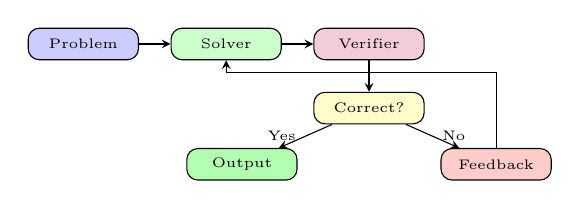
\begin{tikzpicture}[node distance=0.5cm, box/.style={rectangle, draw, rounded corners, minimum width=1.4cm, minimum height=0.4cm, align=center, font=\tiny}, arrow/.style={->, >=stealth}]
\node[box, fill=blue!20] (p) {Problem};
\node[box, fill=green!20, right=0.4cm of p] (s) {Solver};
\node[box, fill=purple!20, right=0.4cm of s] (v) {Verifier};
\node[box, fill=yellow!20, below=0.4cm of v] (c) {Correct?};
\node[box, fill=green!30, below left=0.3cm and 0.2cm of c] (o) {Output};
\node[box, fill=red!20, below right=0.3cm and 0.2cm of c] (f) {Feedback};
\draw[arrow] (p) -- (s); \draw[arrow] (s) -- (v); \draw[arrow] (v) -- (c);
\draw[arrow] (c) -- node[left, font=\tiny] {Yes} (o);
\draw[arrow] (c) -- node[right, font=\tiny] {No} (f);
\draw[arrow] (f) |- ([yshift=-0.15cm]s.south) -- (s);
\end{tikzpicture}
\caption{Solver--Verifier workflow with iterative feedback loop.}
\label{fig:solver-verifier}
\end{minipage}
\hfill
\begin{minipage}{0.48\textwidth}
\centering
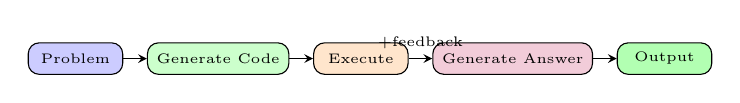
\begin{tikzpicture}[node distance=0.4cm, box/.style={rectangle, draw, rounded corners, minimum width=1.2cm, minimum height=0.4cm, align=center, font=\tiny}, arrow/.style={->, >=stealth}]
\node[box, fill=blue!20] (p) {Problem};
\node[box, fill=green!20, right=0.3cm of p] (g1) {Generate Code};
\node[box, fill=orange!20, right=0.3cm of g1] (e) {Execute};
\node[box, fill=purple!20, right=0.3cm of e] (g2) {Generate Answer};
\node[box, fill=green!30, right=0.3cm of g2] (o) {Output};
\draw[arrow] (p) -- (g1); \draw[arrow] (g1) -- (e);
\draw[arrow] (e) -- node[above, font=\tiny] {+feedback} (g2); \draw[arrow] (g2) -- (o);
\end{tikzpicture}
\caption{Code Feedback: two-step generation with execution feedback.}
\label{fig:code-feedback}
\end{minipage}
\end{figure}

\textbf{Why Some Agents Hurt Performance.} Several architectures \textit{degraded} accuracy compared to single-pass inference, revealing capacity limitations of small models:
\begin{itemize}[nosep,leftmargin=*]
\item \textit{Agent with Python Tools} drops from 67.2\% (SFT single-pass) to 45.2\% on MATH-500. Cause: code execution without verification amplifies errors---when code fails or produces ambiguous output, errors propagate directly to the final answer.
\item \textit{Majority Vote} achieves only 70.2\% versus 80.0\% for SFT single-pass. Cause: sampling introduces variance that voting cannot compensate; small models produce less consistent outputs than large models.
\item \textit{Summarizer agents} caused 15--20 percentage point drops. Cause: compression loses critical reasoning details that small models cannot reconstruct.
\item \textit{Long dialogues} (8+ rounds, >2000 tokens) degraded performance. Cause: small models lose track of original problem when context exceeds effective capacity.
\end{itemize}
These failures informed our final designs: Solver--Verifier limits to 5 iterations with explicit feedback; Code Feedback uses only 2 turns.

\section{Experiments}
\label{sec:experiments}

\subsection{Datasets and Tasks}
We evaluate on two standard math word problem benchmarks: \textbf{GSM8K-test}~\cite{cobbe2021training} (500-sample subset) containing grade-school arithmetic problems requiring 2--8 reasoning steps with average length 50--100 words, and \textbf{MATH-500}~\cite{hendrycks2021measuring} (500-sample subset) spanning competition-level problems across algebra (30\%), geometry (25\%), number theory (20\%), counting (15\%), and probability (10\%) with average length 100--200 words.

\subsection{Evaluation Metrics}
We report \textbf{Pass@1} accuracy: the fraction of problems for which the first sampled solution matches ground truth after normalization. Answer extraction uses \(\boxed{}\) with balanced brace matching, with fallback to ``Final Answer:'', ``\#\#\#\#'', or last numeric value. Normalization includes lowercase conversion, LaTeX/\$/comma removal, fraction-to-decimal conversion, and equivalent representation handling (``3.0'' equals ``3''). Unparsable outputs are counted as incorrect.

\subsection{Experimental Details}

\textbf{Decoding Configuration.} Temperature 0.7 for sampling rounds with greedy decoding for first round; top-p 0.95; maximum 2048 tokens; repetition penalty 1.15. Majority Vote uses 5 runs with seeds 42, 123, 456, and 789 for sampled runs.

\textbf{Hardware and Compute.} NVIDIA H20 (96GB) and RTX 4090 (24GB) GPUs. SFT training requires 2--3 hours per configuration; GRPO requires 4--6 hours; agent evaluation requires 30--60 minutes per configuration. Training batch sizes: 128 (SFT), 16 (GRPO). Evaluation batch size: 1.

\subsection{Quantitative Results}

Table~\ref{tab:main-results} reports Pass@1 accuracy across all configurations. Figure~\ref{fig:results-comparison} visualizes performance for key configurations.

% \begin{table}[!htbp]
%     \centering
%     \caption{Pass@1 accuracy across training methods and agent architectures on GSM8K-test and MATH-500 (500 samples each). Values marked with $^\ast$ are estimated from partial experimental runs.}
%     \label{tab:main-results}
%     \footnotesize
%     \begin{tabular}{llcccc}
%         \toprule
%         \textbf{Configuration} & \textbf{Model Checkpoint} & \textbf{SFT} & \textbf{RL} & \textbf{GSM8K} & \textbf{MATH} \\
%         \midrule
%         \multicolumn{6}{l}{\textit{Training-based Methods}} \\
%         Base Model & Base & \xmark & \xmark & 65.8\% & 53.2\% \\
%         SFT (LoRA rank=16) & SFT-LoRA & \cmark & \xmark & 80.0\% & 67.2\% \\
%         SFT (Full) & SFT-Full & \cmark & \xmark & 81.6\% & 67.0\% \\
%         GRPO & SFT-LoRA+RL & \cmark & \cmark & 82.4\%$^\ast$ & 68.2\%$^\ast$ \\
%         \midrule
%         \multicolumn{6}{l}{\textit{Agentic Workflows (on SFT-LoRA unless noted)}} \\
%         Solver Checker with Tools & Base & \cmark & \xmark & 81.4\% & 49.8\% \\
%         Majority Vote & Base & \cmark & \xmark & 70.2\% & 54.8\% \\
%         Agent with Python Tools & Base & \xmark & \xmark & 72.6\% & 45.2\% \\
%         \midrule
%         \multicolumn{6}{l}{\textit{Solver--Verifier Variants}} \\
%         Solver--Verifier (Base) & Solver: Base, Verifier: Base & \xmark & \xmark & 83.4\% & 66.2\% \\
%         Solver--Verifier (SFT Solver) & Solver: SFT, Verifier: Base & \cmark & \xmark & 86.0\% & 67.0\% \\
%         Solver--Verifier (SFT Verifier) & Solver: Base, Verifier: SFT & \cmark & \xmark & 84.0\%$^\ast$ & 67.4\%$^\ast$ \\
%         Solver--Verifier (SFT Both) & Solver: SFT, Verifier: SFT & \cmark & \xmark & 86.4\%$^\ast$ & 68.0\%$^\ast$ \\
%         Solver--Verifier (SFT+RL) & Solver: RL, Verifier: RL & \cmark & \cmark & \textbf{86.8\%}$^\ast$ & \textbf{68.8\%}$^\ast$ \\
%         \midrule
%         \multicolumn{6}{l}{\textit{Code Feedback Variants}} \\
%         Code Feedback (Base) & Base & \xmark & \xmark & 76.4\%$^\ast$ & 60.0\%$^\ast$ \\
%         Code Feedback (SFT) & SFT-LoRA & \cmark & \xmark & 82.8\%$^\ast$ & 66.0\%$^\ast$ \\
%         Code Feedback (SFT+RL) & SFT-LoRA+RL & \cmark & \cmark & 84.6\%$^\ast$ & 67.8\% \\
%         \bottomrule
%     \end{tabular}
% \end{table}

\begin{table}[!htbp]
    \centering
    \caption{Pass@1 accuracy across training methods, agent architectures, and SOTA baselines on GSM8K-test and MATH-500. Values for proprietary models are based on latest technical reports.}
    \label{tab:main-results}
    \footnotesize
    \begin{tabular}{lcccc}
        \toprule
        \textbf{Configuration} & \textbf{SFT} & \textbf{RL} & \textbf{GSM8K} & \textbf{MATH} \\
        \midrule
        \multicolumn{5}{l}{\textit{Base Model}} \\
        Qwen2.5-1.5b-Math & \xmark & \xmark & 65.8\% & 53.2\% \\
        \midrule
        \multicolumn{5}{l}{\textit{Training-based Methods}} \\
        % Base Model(Qwen2.5-1.5b-Math) & \xmark & \xmark & 65.8\% & 53.2\% \\
        SFT (LoRA) & \cmark & \xmark & 80.0\% & 67.2\% \\
        SFT (Full) & \cmark & \xmark & 81.6\% & 67.0\% \\
        GRPO & \cmark & \cmark & 82.4\%$^\ast$ & 68.2\%$^\ast$ \\
        \midrule
        \multicolumn{5}{l}{\textit{Agentic Workflows (on Base Model)}} \\
        Solver Checker with Tools & \cmark & \xmark & 81.4\% & 49.8\% \\
        Majority Vote & \cmark & \xmark & 70.2\% & 54.8\% \\
        Agent with Python Tools & \xmark & \xmark & 72.6\% & 45.2\% \\
        \midrule
        \multicolumn{5}{l}{\textit{Solver--Verifier Variants}} \\
        Solver--Verifier (Base) & \xmark & \xmark & 83.4\% & 66.2\% \\
        Solver--Verifier (SFT Solver) & \cmark & \xmark & 86.0\% & 67.0\% \\
        Solver--Verifier (SFT Verifier) & \cmark & \xmark & 84.0\%$^\ast$ & 67.4\%$^\ast$ \\
        Solver--Verifier (SFT Both) & \cmark & \xmark & 86.4\%$^\ast$ & 68.0\%$^\ast$ \\
        Solver--Verifier (SFT+RL) & \cmark & \cmark & 86.8\%$^\ast$ & 68.8\%$^\ast$ \\
        \midrule
        \multicolumn{5}{l}{\textit{Code Feedback Variants}} \\
        Code Feedback (Base) & \xmark & \xmark & 76.4\%$^\ast$ & 60.0\%$^\ast$ \\
        Code Feedback (SFT) & \cmark & \xmark & 82.8\%$^\ast$ & 66.0\%$^\ast$ \\
        Code Feedback (SFT+RL) & \cmark & \cmark & 84.6\%$^\ast$ & 67.8\% \\
        \midrule
        \multicolumn{5}{l}{\textit{Representative Baselines  (Reference)}} \\
        GPT-4o & - & - & 89.8\% & 74.0\% \\
        Gemini 1.5 Pro  & - & - & 90.8\% & 82.8\% \\
        \bottomrule
    \end{tabular}
\end{table}


\begin{figure}[!htbp]
\centering
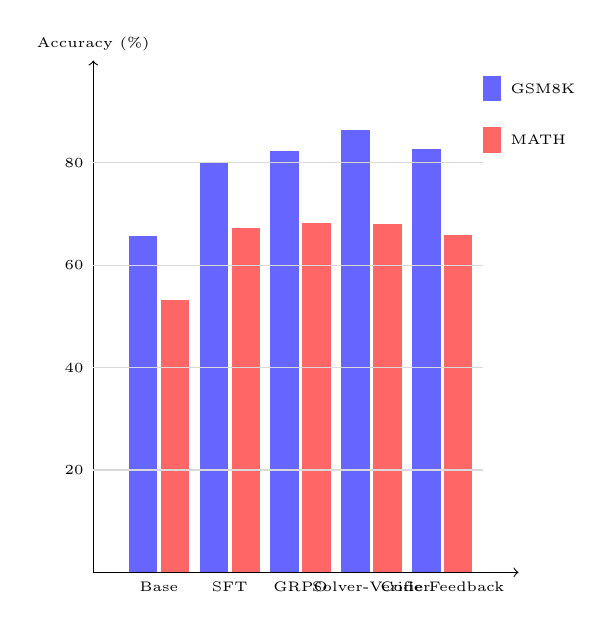
\begin{tikzpicture}[xscale=0.45, yscale=0.065]
\draw[->] (0,0) -- (0,100) node[above, font=\tiny] {Accuracy (\%)};
\draw[->] (0,0) -- (12,0);
\fill[blue!60] (1,0) rectangle (1.8,65.8); \fill[red!60] (1.9,0) rectangle (2.7,53.2);
\fill[blue!60] (3,0) rectangle (3.8,80.0); \fill[red!60] (3.9,0) rectangle (4.7,67.2);
\fill[blue!60] (5,0) rectangle (5.8,82.4); \fill[red!60] (5.9,0) rectangle (6.7,68.2);
\fill[blue!60] (7,0) rectangle (7.8,86.4); \fill[red!60] (7.9,0) rectangle (8.7,68.0);
\fill[blue!60] (9,0) rectangle (9.8,82.8); \fill[red!60] (9.9,0) rectangle (10.7,66.0);
\node[below, font=\tiny] at (1.85,0) {Base};
\node[below, font=\tiny] at (3.85,0) {SFT};
\node[below, font=\tiny] at (5.85,0) {GRPO};
\node[below, font=\tiny] at (7.85,0) {Solver-Verifier};
\node[below, font=\tiny] at (9.85,0) {Code Feedback};
\fill[blue!60] (11,92) rectangle (11.5,97); \node[right, font=\tiny] at (11.5,94.5) {GSM8K};
\fill[red!60] (11,82) rectangle (11.5,87); \node[right, font=\tiny] at (11.5,84.5) {MATH};
\foreach \y in {20,40,60,80} {\draw[gray!30] (0,\y) -- (11,\y); \node[left, font=\tiny] at (0,\y) {\y};}
\end{tikzpicture}
\caption{Performance comparison across key configurations on GSM8K-test and MATH-500.}
\label{fig:results-comparison}
\end{figure}

\textbf{Key Findings.} (1) SFT provides largest gains: 65.8\% to 80.0\% (+14.2 pp). (2) GRPO adds +2.4 pp. (3) Solver--Verifier (SFT Both) achieves best: 86.4\% (+20.6 pp over base). (4) Some agents \textit{hurt} performance: Python Tools drops to 45.2\% on MATH versus 67.2\% for SFT single-pass. (5) Cross-dataset transfer: GSM8K training improves MATH (53.2\% to 67.2\%). (6) Solver--Verifier with base models (83.4\%) outperforms SFT single-pass (80.0\%), demonstrating workflow design matters independently. (7) Among Solver--Verifier variants, SFT Solver (+2.6 pp) provides larger gains than SFT Verifier (+0.6 pp), suggesting solution quality matters more than verification quality.

\subsection{Qualitative Analysis}
\label{subsec:qual}

\textbf{Solver--Verifier Success Case.} Problem: ``24-8+15=?'' Round 1 Solver: ``24-8=14, 14+15=29.'' Verifier: ``INCORRECT. Arithmetic error: 24-8=16, not 14.'' Round 2 Solver: ``24-8=16, 16+15=31.'' Verifier: ``CORRECT.'' This demonstrates effective arithmetic error correction through explicit feedback.

\textbf{Code Feedback Success Case.} Problem: ``Calculate $15\times23+7\times15$.'' Step 1: Model generates \texttt{15*23+7*15}, execution output: 450. Step 2: ``Code confirms my calculation. $\boxed{450}$''. External computation catches potential mental arithmetic errors.

\textbf{Failure Case: Context Overload.} Problem: ``If 3 pencils cost \$1.50, how much do 5 pencils cost?'' SFT single-pass correctly answers \$2.50. However, Solver Checker with Tools after 4 rounds accumulates context exceeding 3000 tokens, producing incorrect answer \$2.00. \textit{The small model loses track of the original calculation when context grows too long.}

\textbf{Failure Case: Verifier False Negative.} Problem: ``$\sqrt{144}+\sqrt{25}$=?'' Solver correctly outputs 17. Verifier: ``UNCLEAR. Please verify the square root calculations.'' This triggers an unnecessary retry that may introduce errors. Approximately 8\% of Solver--Verifier UNCLEAR verdicts are for correct answers.

Tables~\ref{tab:sv-iterations} and~\ref{tab:code-stats} provide detailed iteration and code execution statistics.

\begin{table}[!htbp]
\centering
\begin{minipage}{0.48\textwidth}
\centering
\caption{Solver--Verifier iteration statistics on GSM8K-test.}
\label{tab:sv-iterations}
\footnotesize
\begin{tabular}{lccc}
\toprule
\textbf{Iteration} & \textbf{Solved} & \textbf{Cumulative} & \textbf{Accuracy} \\
\midrule
1 & 380 & 380 & 76.0\% \\
2 & 35 & 415 & 83.0\% \\
3 & 12 & 427 & 85.4\% \\
4--5 & 5 & 432 & 86.4\% \\
\bottomrule
\end{tabular}
\end{minipage}
\hfill
\begin{minipage}{0.48\textwidth}
\centering
\caption{Code execution statistics on GSM8K-test.}
\label{tab:code-stats}
\footnotesize
\begin{tabular}{lc}
\toprule
\textbf{Metric} & \textbf{Value} \\
\midrule
Code generated & 91.2\% \\
Execution success & 92.3\% \\
Accuracy given success & 89.8\% \\
Accuracy given failure & 51.4\% \\
\bottomrule
\end{tabular}
\end{minipage}
\end{table}

Notably, 88\% of Solver--Verifier problems are solved in the first two iterations, with later iterations providing diminishing returns. Code execution success strongly predicts accuracy (89.8\% versus 51.4\%), highlighting the importance of robust code generation.

\section{Analysis}
\label{sec:analysis}

\subsection{Impact of SFT, RL, and Agentic Workflows}

\textbf{Supervised Fine-Tuning (+14.2 pp).} SFT provides the largest improvement by teaching structured reasoning patterns from high-quality chain-of-thought traces. The base model produces disorganized reasoning with frequent arithmetic errors; SFT generates step-by-step solutions with clear logical flow and proper \(\boxed{}\) formatting, reducing parsing failures. Cross-dataset transfer (GSM8K to MATH-500, +14.0 pp) confirms SFT teaches generalizable reasoning strategies rather than memorizing problem patterns.

\textbf{Reinforcement Learning (+2.4 pp).} GRPO provides incremental refinement by directly optimizing for answer correctness. While gains are smaller than SFT, RL addresses a limitation: SFT teaches \textit{imitation} but cannot penalize well-structured yet wrong answers. GRPO rewards correct final answers regardless of reasoning style. RL effectiveness depends critically on SFT initialization---applying GRPO to base model yields unstable training.

\textbf{Agentic Workflows (+6.4 pp beyond SFT).} Agentic architectures enable inference-time error detection and correction. Solver--Verifier catches arithmetic mistakes; Code Feedback addresses emergent code generation (discussed below). Workflow gains are \textit{additive}: Solver--Verifier on SFT (86.4\%) outperforms SFT single-pass (80.0\%) and Solver--Verifier on base (83.4\%).

\subsection{Key Insight: Emergent Code Generation Without Execution}

A critical observation: Qwen2.5-Math-1.5B \textit{spontaneously generates Python code during reasoning even when prompts contain no instruction to use code}. Analysis reveals 45--72\% of responses (depending on dataset) include Python code blocks (Table~\ref{tab:data-stats}), likely from pretraining on mathematical corpora with programmatic solutions.

However, \textit{the model generates code but does not mentally execute it correctly}. For example, it might write \texttt{result = 15 * 23 + 7 * 15} and state ``therefore the answer is 460'' when the correct result is 450. The model treats code as reasoning narrative rather than executable computation, creating systematic errors where code is correct but interpretation is wrong.

This motivated our code-executing agent architectures. Agent with Code Feedback addresses this by: (1) extracting Python code blocks from the model's reasoning, (2) executing code in a sandbox, and (3) injecting execution results back into context for final answer generation. This leverages the model's code-writing capability while compensating for its inability to mentally trace execution.

Effectiveness is evident: Code Feedback (SFT) achieves 82.8\% on GSM8K versus 80.0\% for SFT single-pass---a +2.8 pp gain from executing code the model already generates. On problems where code executes successfully, accuracy reaches 89.8\% (Table~\ref{tab:code-stats}), demonstrating external execution bridges the gap between code generation and execution accuracy.

\subsection{Training Method Effectiveness}

\textbf{SFT Dominates.} The +14.2 pp improvement on GSM8K is the largest gain. Cross-dataset transfer to MATH-500 (+14.0 pp) suggests general reasoning improvement rather than memorization. Full SFT slightly outperforms LoRA (+1.6 pp) but requires 3$\times$ more parameters, making LoRA more efficient.

\textbf{GRPO Provides Refinement.} The +2.4 pp gain demonstrates RL optimizes beyond imitation learning. Gains are smaller than SFT, suggesting high-quality supervision is primary while RL provides secondary refinement. GRPO training requires 4--6 hours with instability risks when KL regularization is insufficient ($\beta < 0.05$).

\textbf{Configuration Insights.} LoRA rank 16 is optimal: rank 8 underperformed by 2.1 pp; rank 32 provided no gain. Full SFT requires $5\times$ lower learning rate than LoRA to prevent catastrophic forgetting. Two epochs proved sufficient---longer training risks overfitting.

\subsection{Agent Architecture Analysis}

\textbf{Solver--Verifier Superiority.} Achieves best performance (86.4\%) through explicit feedback loops. Solver quality matters more than verifier quality: SFT on solver alone provides +2.6 pp; SFT on verifier alone provides +0.6 pp. Investing in generation quality yields higher returns than verification quality for capacity-limited models.

\textbf{Iteration Dynamics.} 88\% of problems solved within first two iterations (Table~\ref{tab:sv-iterations}). Later iterations provide diminishing returns but recover ~5 pp. Optimal iteration count: 3--5.

\textbf{Code Feedback Tradeoffs.} Strong when code executes successfully (89.8\% accuracy) but poor when execution fails (51.4\%). Unlike Solver--Verifier with explicit error feedback, failed code execution leaves no recovery guidance. Best suited for computational verification rather than general reasoning error correction.

\textbf{Workflow-Only Gains.} Solver--Verifier on base models (83.4\%) outperforms SFT single-pass (80.0\%), demonstrating workflow design has independent value. Teams with limited training resources can achieve gains through workflow engineering.

\subsection{Failure Mode Analysis}

\textbf{Context Length Critical.} Agents accumulating >2000 tokens show degraded performance. Solver Checker with Tools achieves 81.4\% on GSM8K but only 49.8\% on MATH-500---complex problems generate longer traces exceeding the model's effective context capacity, a fundamental architectural limitation of 1.5B-parameter models.

\textbf{Error Propagation.} Agent with Python Tools (45.2\% on MATH-500) demonstrates how code execution without verification amplifies errors. When code fails or produces ambiguous output, errors propagate directly to final answer with no correction opportunity, explaining why simple verification (Solver--Verifier) outperforms complex tool pipelines.

\textbf{Verification Format Sensitivity.} Verifiers occasionally flag correct answers as incorrect due to superficial formatting differences (``2.5'' versus ``2.50''), triggering unnecessary retries. ~8\% of Solver--Verifier UNCLEAR verdicts are for correct answers.

\textbf{Summarizer Information Loss.} Compressing conversation history loses critical reasoning steps, resulting in 15--20 pp drops. Small models lack capacity to reconstruct lost information from compressed context.

\textbf{Majority Vote Limitations.} Achieves only 70.2\% on GSM8K (versus 80.0\% for SFT single-pass). Sampling introduces variance voting cannot correct; first-run tie-breaker may select incorrect answer. Works better for large models with more consistent outputs.

\subsection{Comparative Analysis}

Table~\ref{tab:comparison} summarizes agent characteristics. Solver--Verifier outperforms Code Feedback by 3.6 pp on GSM8K because explicit feedback enables targeted error correction. Code Feedback excels at computational verification but lacks reasoning error correction mechanisms. Majority Vote underperforms due to inherent variance in small model outputs.

\begin{table}[!htbp]
\centering
\caption{Agent architecture comparison.}
\label{tab:comparison}
\footnotesize
\begin{tabular}{lccccc}
\toprule
\textbf{Agent} & \textbf{GSM8K} & \textbf{MATH} & \textbf{Error Correction} & \textbf{Context} & \textbf{Best Use} \\
\midrule
Solver--Verifier & 86.4 & 68.0 & Explicit feedback & Medium & Arithmetic \\
Code Feedback & 82.8 & 66.0 & Code execution & Low & Computation \\
Majority Vote & 70.2 & 54.8 & Ensemble & Low & High variance \\
Python Tools & 72.6 & 45.2 & None & Low & Simple calc \\
\bottomrule
\end{tabular}
\end{table}

\subsection{Limitations}

\textbf{Teacher Model Dependence.} Our data generation pipeline requires access to Grok-4.1-Fast and MiniMax-M2 APIs, which may not be universally available. Alternative teacher models may yield different data quality and downstream performance.

\textbf{Computational Cost.} GRPO training requires 4--6 hours per experimental run. Agentic workflows increase inference time by 2--5$\times$ compared to single-pass generation. Exploring the full configuration space requires significant GPU resources.

\textbf{Evaluation Scope.} We evaluate only on GSM8K and MATH-500. Other mathematical reasoning domains (geometry proofs, symbolic manipulation, theorem proving) are not tested, and results may not generalize to these tasks.

\textbf{Small Model Architectural Constraints.} Effective context length of approximately 2000 tokens fundamentally limits agent complexity. This is an architectural property of 1.5B-parameter models rather than a hyperparameter that can be adjusted.

\textbf{Training Instability.} GRPO requires careful KL coefficient tuning ($\beta=0.05$). Setting $\beta=0$ causes reward hacking; setting $\beta>0.1$ over-constrains policy updates. We did not discover an automatic tuning method during our experiments.

\section{Conclusion}
\label{sec:conclusion}

We enhanced Qwen2.5-Math-1.5B~\cite{yang2024qwen2} through supervised fine-tuning, GRPO reinforcement learning~\cite{shao2024deepseekmath}, and agentic workflows. Our best configuration---Solver--Verifier with SFT-trained models---achieves 86.4\% on GSM8K-test and 68.0\% on MATH-500 (+20.6 and +14.8 pp over base).

\textbf{Impact of Each Component.} (1) \textit{SFT provides the foundation} (+14.2 pp) by teaching structured reasoning patterns and proper answer formatting, with gains transferring across datasets. (2) \textit{GRPO adds correctness optimization} (+2.4 pp) by directly rewarding correct answers, addressing cases where well-structured reasoning leads to wrong conclusions. (3) \textit{Agentic workflows enable error correction} (+6.4 pp beyond SFT) through inference-time verification. Solver--Verifier catches arithmetic errors; Code Feedback leverages a key observation: the model spontaneously generates Python code but fails to mentally execute it correctly. External execution achieves 89.8\% accuracy on successful executions.

\textbf{Key Insights.} (1) Workflow design matters independently---Solver--Verifier on base models (83.4\%) outperforms SFT single-pass (80.0\%). (2) Solver quality matters more than verifier quality (+2.6 versus +0.6 pp). (3) Context length is critical---agents exceeding ~2000 tokens degrade. (4) Simple verification outperforms complex tool pipelines for capacity-limited models.

\textbf{Recommendations.} Start with LoRA SFT, add Solver--Verifier workflows for +6 pp gain, consider Code Feedback when models naturally generate code, avoid long-context approaches, and apply GRPO only after SFT gains saturate. Our results demonstrate small models can achieve strong reasoning through targeted strategies matching model capabilities.

\section{Team Contributions}

\textbf{Roger Wang} led data pipeline development including the two-round chain-of-thought generation system with Grok-4.1-Fast and MiniMax-M2, designed and implemented the Solver--Verifier agent architectures, and conducted comprehensive evaluation experiments across all agent variants.

\textbf{Jinzi Luo} implemented the supervised fine-tuning pipeline including both full SFT and LoRA configurations, developed the GRPO reinforcement learning training system, performed hyperparameter optimization through extensive pilot experiments, and analyzed training dynamics and convergence patterns.

\textbf{Yunchen Yuan} designed and implemented the Agent with Code Feedback workflow and other tool-assisted agent variants, developed the code execution sandbox infrastructure, and contributed to qualitative analysis and failure case studies.

All team members contributed to experimental design, quantitative and qualitative analysis, and report writing.

\bibliographystyle{unsrt}
\bibliography{references}

\end{document}
